\section{Ограничения}
\label{sec:limitations}

Настоящая работа имеет ряд ограничений, которые мы структурируем по четырём осям: эпистемологические, измерительные, дизайн-связанные, статистические. Эти ограничения --- не ретроспективный подстройщик претензий, а явная граница того, что данные поддерживают, и что --- нет.

\subsection{Картина мира как первичный источник рамки}
\label{subsec:worldview_first}

DEIC-программа построена \emph{worldview-first}, и этот порядок мы считаем обязательным назвать открыто. Картина того, как устроена архитектура эмпатии и не-эмпатии, сложилась у авторов до сбора данных --- из психоаналитической традиции, клинического наблюдения и материала контемплативных источников; 131-пунктный инструмент был сконструирован специально, чтобы эту картину проверить. Это не анти-паттерн: большинство содержательных теоретических синтезов в психологии (теория привязанности у \citealp{bowlby1969}, mentalization theory у \citealp{fonagy2002}, клиническая традиция психопатии от \citealp{cleckley1941} к \citealp{hare1991}) построены ровно так же, и «данные первичны, теория вторична» остаётся риторической позицией, которая редко совпадает с реальным процессом. Мы считаем более честным назвать этот порядок, чем замаскировать его под обратный.

Из worldview-first структуры вытекают три специфических риска, требующих прямой дисклоужер.

\paragraph{Риск конфирмации.} Автор рамки имеет свободу в выборе инструмента, спецификаций моделей, способа агрегации и интерпретации и может бессознательно оптимизировать эти решения под подтверждение исходной интуиции. Защита --- пре-регистрированная репликация на независимой выборке, собранная и анализированная исследователем, не вовлечённым в разработку рамки и методологически склонным к её опровержению. Без этого шага текущая работа должна читаться как развёрнутая гипотеза, подкреплённая одной выборкой, а не как установленный факт.

\paragraph{LLM как структурный усилитель рамки.} Значительная часть работы по уточнению конструктов, формулировке теоретических связок и компоновке итогового каркаса велась в диалоге с большими языковыми моделями. Это методологически значимо не из-за галлюцинаций (в концептуальной работе они пренебрежимы), а из-за асимметрии сопротивления. LLM без собственной биографии, без защитной структуры и без источника scepticисм вне предоставленной ей рамки --- не скептический коллега, а логически когерентный резонатор: он продлевает исходную рамку в те места, где живой собеседник остановился бы и сказал «погоди». Отсутствие трения здесь --- не отсутствие коррекции, а активное усиление. Частичная компенсация --- живой диспут с методологически трезвым оппонентом, не разделяющим рамку, --- должна быть встроена в подготовку волны~2 и явно зафиксирована в методологии.

\paragraph{Три кардинальных условия фальсификации.} Рамка осмысленна только если она платит цену. Мы формулируем три кардинальных условия, отказ от которых разрушает соответствующие части программы.

\emph{(a) Возрастная инвариантность канала CA$\to$ID$\to$\EAF{} в диапазоне 14--45 лет.} Если в независимой репликации параметры канала значимо зависят от возраста в этом диапазоне, тезис о критическом окне формирования архитектуры до 14 лет не держится, и архитектурно-онтогенетическая интерпретация программы теряет основание.

\emph{(b) Ортогональность P$\perp$CA на популяционном уровне.} Если в репликации корреляция P с CA значимо положительна или indirect effect CA$\to$P$\to$\EAF{} значимо ненулевой, двухслойная структура P (архитектура $+$ моральный нарратив, независимые от детской истории) не держится, и модель возвращается к стандартной клинической рамке «психопатия как последствие травмы».

\emph{(c) Воспроизводимость первичного кластера (hi-P, lo-CA, lo-ID).} В текущих данных он выделился rule-based классификацией как $n = 144$ (10\% выборки). Если в независимой репликации он не выделяется или его размер радикально меньше, различение первичного и вторичного паттернов возвращается к статусу теоретического предположения, и тезис о двух этиологических путях к условной архитектуре не подтверждается.

Эти три условия --- не символический жест, а реальная дорогостоящая ставка: отказ хотя бы от одного потребует переформулировки центральной части рамки. Вместе с тремя точками эмпирического сопротивления, уже наблюдавшимися в текущей выборке (§\ref{subsec:data_resistance}), они образуют минимальный набор проверок, который делает DEIC фальсифицируемой программой, а не самоподтверждающейся рамкой.

\subsection{Измерительные ограничения}

\paragraph{A как формативный, не рефлексивный конструкт.} Это ограничение подтверждено эмпирически в A-CFA Tier 5. На 17 тщательно отобранных метакогнитивных айтемах CFI $= 0.866$, RMSEA $= 0.081$, $\omega$ по абсолютным нагрузкам $= 0.947$, но загрузки \emph{биполярные} --- 8 положительных, 9 отрицательных после внешнего выравнивания полярности. Когда этот латентный A подставляется в conditional process SEM, знаки переворачиваются относительно теоретически взвешенного композита (A$_{\mathrm{lat}} \to$ ID $= +0.66$ вместо композитного $-0.63$), и \IMM{} $= -0.00044$ [$-0.00267, +0.00052$] незначим. Это не провал анализа, а эмпирическое доказательство того, что текущий пул айтемов не различает witnessing (наблюдение-наблюдения) от trauma hypervigilance (болезненной гипервнимательности к внутренним состояниям). Главный композит работает потому, что мы заранее вложили это различие в веса. Dedicated A-scale --- приоритет номер один в волне 2.

\paragraph{M-фактор низкой надёжности.} $\omega = 0.546$ против $\omega > 0.89$ у остальных пяти факторов. Masking слабо дифференцирован от P ($r_{\mathrm{latent}} = +0.82$). M-специфические выводы в статье не делаются; M вынесен как регуляторный слой для пересборки в волне 2.

\paragraph{Post-hoc статус ACE-расширения.} Расширение ACE-конструкта (трактовка «не помню / не знаю» как позитивного сигнала адверсивно-релевантной семейной или когнитивной конфигурации вместо missing data) обсуждается содержательно в §\ref{subsec:ace_extension} и валидировано на wave-1 через полный 6-factor oblique CFA re-fit (N~$=$~1468 против канонических 1426; CFI~$=$~0.960, RMSEA~$=$~0.062; bootstrap~95\%~CI индиректов не пересекают ноль). Тем не менее эта валидация \emph{post-hoc}: переключение кодировки и re-fit произведены после исходной публикационной CFA. Pre-registered wave-2 с изначально-спроектированной ACE-dissociation подшкалой и с заранее заявленными критериями (McDonald's $\omega \ge 0.7$, $r(\text{ACE-dis}, \text{ID}_{\mathrm{lat}}) \ge 0.30$) --- условие превращения расширения из наблюдения в утверждение о репродуцируемой структуре. См. §\ref{sec:future}.

\paragraph{Сворачивание wave-1 шкал в текущую шестифакторную структуру.} Инструмент-прародитель (DEIC-Inventory wave-1) имел 12 содержательных шкал $+$ 2 контрольных (A, Lie). Публикуемая шестифакторная oblique-CFA-модель --- результат двух психометрически вынужденных операций сворачивания и одной операции расщепления.

\emph{Сворачивание защит (пять в одну, с сохранением концептуального центра).} Wave-1 имел пять шкал пассивного блокирования: четыре mechanism-specific --- подавление (\texttt{S}), диссоциация (\texttt{D}), аффективная изоляция (\texttt{AIS}), аффективная уплощённость (\texttt{F}) --- и одну experiential-центральную --- \emph{Internal Dissonance Scale} (\texttt{IDS}), измеряющую субъективное переживание «эмпатический отклик запущен, но дальше не идёт; хочу чувствовать, но не могу». Выбор в пользу единого ID-латента в основной модели --- решение о \emph{парсимонии}, а не приговор структуре: на наших данных пятифакторная oblique-CFA сходится (CFI~=~0.891, RMSEA~=~0.077), но латентные корреляции между пятью защитами имеют $|r|$ в диапазоне $0.66$--$0.89$ с частично противоположными знаками (структура с mixed signs, характерная для полу-свёрнутой коллинеарности). На этом уровне разделимости пять отдельных латентов не дают клинически и статистически устойчивого различения; одновременно --- общий ID-латент поглощает большую часть варьирования. Wave-2 (настоящая работа) сохраняет концептуальный центр без изменений и просто убирает «Scale» из обозначения: \texttt{IDS} $\to$ \textbf{ID} (\emph{Internal Dissonance}). Расширение же состоит в том, что четыре mechanism-specific шкалы (S, D, AIS, F) свёрнуты внутрь того же латента как поверхностные манифестации поля. Содержательно это согласуется с Фонаги (отсутствие ментализирующего поля как условие, а не сумма механизмов) и с Di Giuseppe \& Perry~\citep{digiuseppe2024} (защиты как интегрированная сеть, а не параллельные черты).

\emph{Ограничение парсимонии.} Поглощение не равносильно доказательству одномерности. В дополнительном bifactor-анализе (§\ref{subsec:id_bifactor}) общая факторная модель (ID\textsubscript{g} плюс пять uncorrelated specific-factors) превосходит унифакторную ID-модель по основным индексам и показывает, что общий ID объясняет около 57\% общей дисперсии (ECV\textsubscript{global}~=~0.57), при заметной гетерогенности per-subscale: FLA и IDS почти полностью поглощаются общим ID (ECV~=~0.86 и 0.66 соответственно), DIS и AIS держат около половины уникальной дисперсии (ECV~$\approx$~0.54, 0.53), а SUP остаётся в значительной мере отдельным конструктом (ECV~=~0.31). Клинически это означает: подавление (SUP) хуже всех поглощается umbrella-латентом и в волне~2 с высокой вероятностью должно быть восстановлено как отдельный латент; FLA --- наоборот, хорошо описывается общим ID и может остаться его надёжным индикатором; DIS и AIS стоят посередине --- требуют либо дополнительных айтемов для чистой сепарации, либо bifactor-уровня в публикуемой модели. Феноменологические различия между surface-механизмами --- подавление (эго-синтонное сознательное), диссоциация (эго-дистонное автоматическое), аффективная изоляция (содержание присутствует, чувство отрезано), уплощённость (аффективный сигнал отсутствует) --- в публикуемой унифакторной ID-модели спрятаны; в bifactor-модели и в wave-2-дизайне они восстанавливаются.

\emph{Сворачивание контекстуального слоя (ACE $+$ CA $\to$ CA).} Wave-1 различал общий индекс неблагоприятного детского опыта (\texttt{ACE} в духе Felitti et al.) и узкую шкалу childhood adversity (\texttt{CA}, акцент на реляционной травме ранних лет). На нашей выборке они оказались взаимозаменяемыми индикаторами одного латента ($r > 0.8$), поэтому в публикуемой модели используется единый \textbf{CA} как латент ранней реляционно-стрессовой истории. Wave-1 различение типов травмы (бытовое насилие, эмоциональная депривация, нестабильность привязанности) в этой агрегации скрыто. Дополнительные контекстуальные шкалы wave-1 --- эмоциональный контекст (\texttt{EC}) и аффективно-диссоциативный индикатор (\texttt{ADI}) --- сохранены как наблюдаемые композиты для дескриптивного использования, но не входят в основной CFA как латенты.

\emph{Расщепление эмпатии (одна в две).} Противоположная операция: wave-1 общая шкала эмпатии \texttt{E} разделена на \EAF{} и \Ecog{} post-hoc, в ответ на парадокс P$\leftrightarrow$E в оригинальной модели и в согласии с многомерной традицией Davis~\citep{davis1983}. Это приобретение, а не потеря; но оно post-hoc и должно быть воспроизведено на pre-registered айтемах, разведённых по дизайну (см. ниже --- статистические ограничения).

\begin{figure}[htbp]
\centering
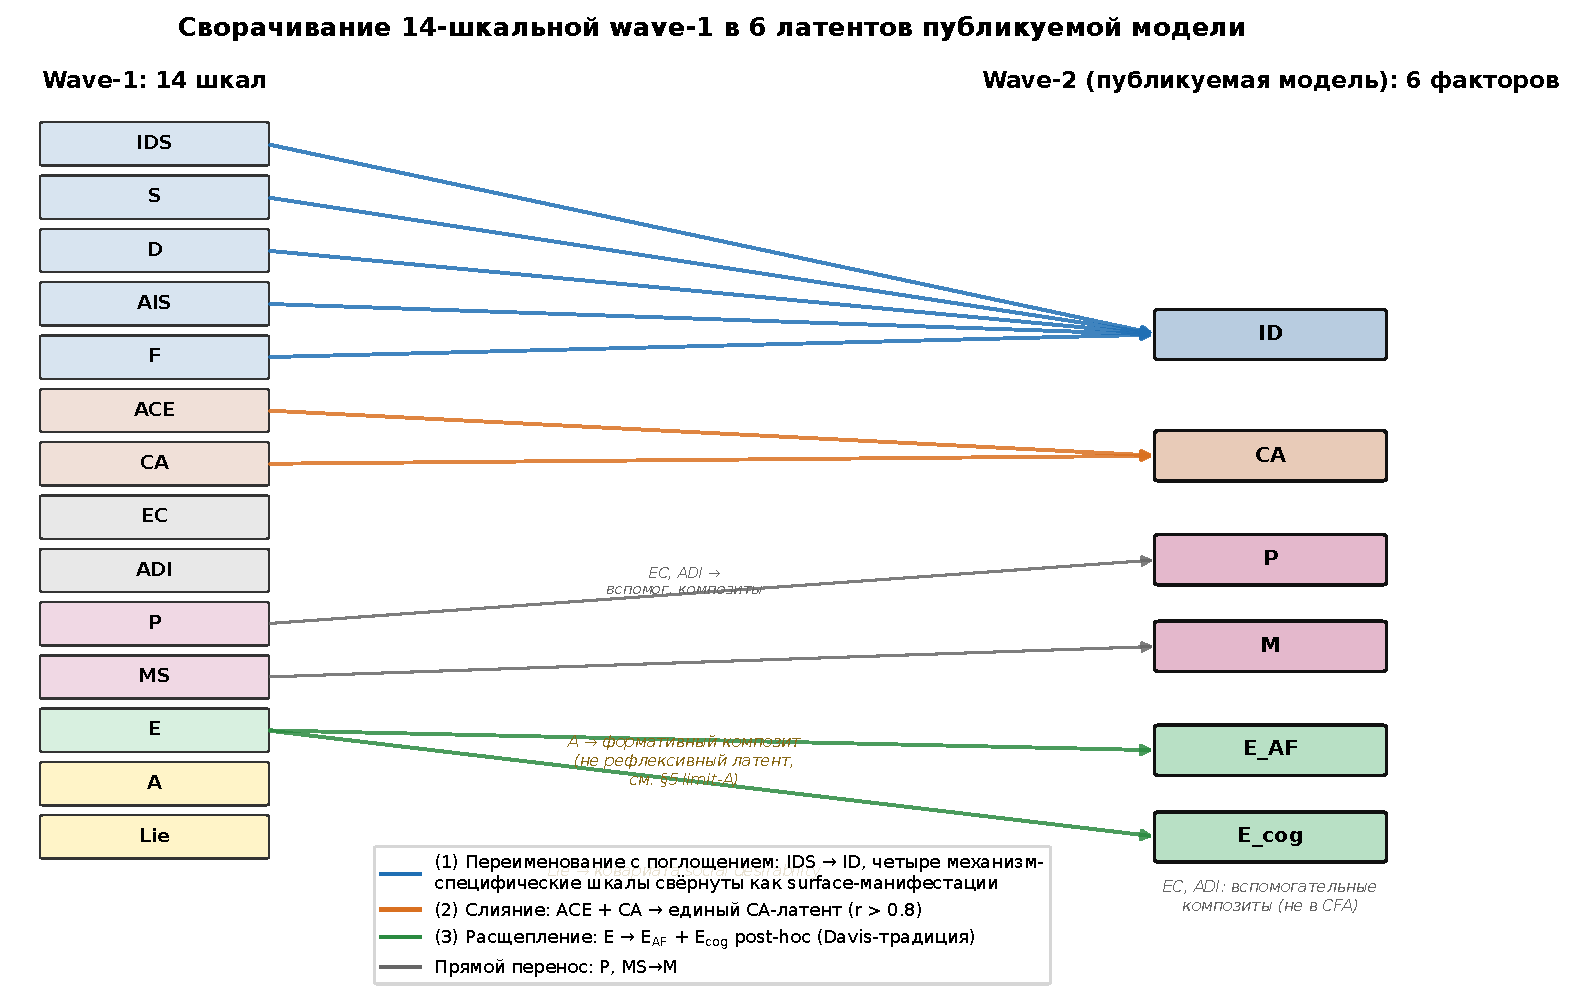
\includegraphics[width=0.95\linewidth]{figures/fig9_wave_mapping.pdf}
\caption[Карта перехода wave-1 $\to$ wave-2]{Карта перехода от 14 wave-1 шкал к 6 латентам публикуемой модели. Синие стрелки --- переименование с поглощением (IDS $\to$ ID, вместе с S, D, AIS, F как surface-манифестации одного поля); оранжевые --- слияние двух индикаторов ранней истории (ACE + CA $\to$ CA); зелёные --- расщепление общей шкалы эмпатии (E $\to$ \EAF{} + \Ecog{}); серые --- passthrough (P, MS $\to$ M). EC, ADI сохранены как вспомогательные наблюдаемые композиты; A, Lie --- контрольные шкалы.}
\label{fig:wave_mapping}
\end{figure}

\emph{Итоговая карта.} 12 содержательных wave-1 шкал $\to$ 6 латентов публикуемой модели: \texttt{IDS} $\to$ \textbf{ID} (переименование с поглощением \{\texttt{S, D, AIS, F}\} как неотделимых surface-манифестаций того же поля); \{\texttt{ACE, CA}\} $\to$ CA (объединение двух индикаторов ранней реляционной истории в единый латент); \texttt{P} $\to$ P; \texttt{MS} $\to$ M; \texttt{E} $\to$ \{\EAF, \Ecog\} (post-hoc расщепление, единственная операция расширения); \{\texttt{EC, ADI}\} $\to$ вспомогательные наблюдаемые композиты. A отделена как формативный композит; Lie --- ковариата social desirability, корректирующая E и ID в прикладных интегральных метриках. Публикуемая шестифакторная структура --- минимальная, которую данные поддерживают. Феноменологические и типологические различия, спрятанные в этой минимальности, --- задача волны 2.

\paragraph{Multi-scale веса в \texttt{questions.json} --- новация и её scoring-артефакт.} Эксплицитное a-priori приписывание каждому айтему вектора весов по нескольким факторам --- существенная содержательная новация инструмента, а не методологическая небрежность: большинство опросников эмпатии делают вид, что simple structure справедлива, и приписывают айтем одной шкале, теряя ту часть дисперсии, которая сидит на пересечениях конструктов. DEIC этот cross-структурный аспект выносит из неявных статистических артефактов в явную теоретическую декларацию, которую можно критиковать и валидировать (ближайший психометрический родственник --- a-priori bifactor-модели). Однако композитное sum-scoring с multi-scale весами алгебраически раздувает корреляции между композитами: пункт с ненулевыми весами в двух композитах засчитывается с обеих сторон уравнения, когда эти композиты коррелируют. В нашей выборке средняя инфляция $\sim 0.18$, максимум $0.68$ с переменой знака P$\leftrightarrow$E. Латентные факторные скоры этой проблемы лишены, потому что CFA корректно разделяет общую и специфичную дисперсию. Wave-2 решение --- не отказ от новации, а её разделение на два независимых слоя в \texttt{questions.json}: \texttt{factor\_weights} (вектор для CFA с явно прописанными cross-loadings --- теоретический слой остаётся) и \texttt{primary\_scale} (единственный фактор для композитного sum-scoring --- один айтем, один композит). Композиты публикуются как ориентировочные без алгебраической инфляции; латентные скоры --- как основной научный результат. Новация сохраняется в полном объёме и становится двухуровневой по конструкции.

\paragraph{Self-report only.} Нет informant-report, нет поведенческих мер, нет физиологических конвергентных измерителей. Особенно критично для A, где self-report имеет circular-validity ограничение (точный отчёт о внимании требует внимания).

\paragraph{Вторичная психопатическая подгруппа мала.} $n = 65$. Rule-based $2 \times 2$ даёт устойчивое направление, но величины эффектов во вторичной ячейке имеют широкие CI и требуют клинической выборки для подтверждения.

\subsection{Дизайн-связанные ограничения}

\paragraph{Cross-sectional.} Нет временной оси, нет pre/post-терапевтического дизайна, нет retest-стабильности. Следствие: невозможно различить стабильный A от транзиторного, невозможно тестировать longitudinal-предсказания, сформулированные в §\ref{subsec:falsifiers}, и невозможно эмпирически различить direction of causation в паре CA--ID (теоретически предполагаемая, но статистически неидентифицированная).

\paragraph{Моноязычная выборка.} Русскоязычный интернет-рекрутинг; выборка self-selected. Культурный, языковой и платформенный bias присутствуют. Cross-cultural валидация (EN, ES, CH, AR) с invariance-testing --- обязательный следующий шаг.

\paragraph{Возрастной перекос} в сторону 18--37; подгруппа 38+ ($n = 50$) мала. Супрессорная медиация устойчива на 18--37, ослабевает 38+; механизм неясен --- post-therapy effects, survivor bias, developmental shift --- и требует возраст-стратифицированной выборки.

\paragraph{Self-selection через Telegram/VK.} Опросник требует intro-метакогнитивного vocabulary; возможно, эта форма селекции уже сдвигает распределение A вправо относительно генеральной популяции. Данные не поддерживают распространение на non-reflexive субпопуляции.

\paragraph{Подвыборка «befriends-psychopaths» и этика индивидуального уровня.}
\label{subsec:limitations_befriends}
Архетип эмпатического контрагента в диаде с психопатом (hi-E $+$ hi-P в октанте $+++-$) эмпирически подтверждён, но представлен в выборке только $n = 3$ респондентами ($0.19\%$). Никто из них не отметил ни одной текстовой диагностической категории, самоописания этого профиля в свободном поле отсутствуют: архетип систематически невидим для self-report. Ретроспективная power-оценка: детектирование $d = 0.5$ в этой подгруппе требует $n \approx 150$, $d = 1.0$ --- $n \approx 30$. В текущей волне профиль зафиксирован описательно, без параметрических сравнений. Wave~2 требует целенаправленного сэмплинга этой конфигурации. \emph{Этическое ограничение:} один из трёх респондентов известен нам биографически, поэтому любые индивидуальные характеристики этой подгруппы публикуются только как агрегированные центроиды ($n = 3$); индивидуальный уровень данных из статьи исключён и не передаётся в открытые supplementary.

\subsection{Статистические ограничения}

\paragraph{Многомерная не-нормальность данных и robust fit indices.} Mardia $p < 0.0001$. Реализованы две приближённые robust-пересчётки. \textbf{(а)}~Bootstrap-аппроксимация Satorra--Bentler scaling (в \texttt{tier4\_analyses.py}). \textbf{(б)}~Satorra--Bentler T$_1$ через \texttt{semopy.stats.calc\_chi2\_sb} с четвёрто-моментной весовой матрицей из \texttt{prepare\_wls} поверх ML-посадки: $\chi^2_{\mathrm{SB}}(120) = 934.25$, CFI$_{\mathrm{SB}} = 0.873$, RMSEA$_{\mathrm{SB}} = 0.098$, scaling factor $c = 0.552$. Нетипичное $c < 1$ (ML-$\chi^2$ дефлирован относительно SB-корректированного) и падение CFI с $0.950$ до $0.873$ --- два независимых сигнала, что содержательные выводы статьи следует оценивать на latent factor scores (устойчивых к этой коррекции), а не на глобальных fit-индексах. Точные MLR SE и WLSMV на сырых ordinal-айтемах требуют \texttt{lavaan} в R для финальной публикации; это инфраструктурный gap, а не содержательный, и reviewer-стандарт его требует эксплицитно.

\paragraph{Conditional process SEM на композитном модераторе A.} После A-CFA корректная реализация --- переход к структурному моделированию A как латента, с учётом его биполярной природы. В текущей форме A-модерация держится на теоретически взвешенном композите; это работает, но требует дублирования в структурной форме.

\paragraph{Post-hoc характер факторного разделения \EAF{}/\Ecog{}.} Разделение когнитивной и аффективной эмпатии было установлено post-hoc в ответ на парадокс P$\leftrightarrow$E в оригинальной модели. Pre-registered replication с айтемами, разведёнными по дизайну, --- необходимое условие для устойчивости этого различения.

\subsection{Теоретические гапы}

Это не ограничения текущей статьи в строгом смысле, а \emph{отсутствующие элементы в теории}, которые программе предстоит заложить. Мы их перечисляем явно, потому что граница известного --- часть эмпирической работы.

\paragraph{Временной каркас.} Теория в текущем виде --- cross-sectional snapshot. Вся содержательная лексика («автоматизм», «осознанность») --- temporal. Требуется трёхшкальный временной фрейм: fast (ms--s, стимул $\to$ активация ID $\to$ подавление \EAF{}), meso (недели--месяцы, repeated A-активации в терапии $\to$ постепенное расцепление), slow (годы--декады, ACE $\to$ формирование ID-паттерна $\to$ рекрутирование P или нет). Планируется отдельная статья «\DEIC{} dynamics: temporal architecture of empathy blocking».

\paragraph{Механизм переключателя ID $\leftrightarrow$ P.} Эмпирически ID и P разделимы. Но \emph{что решает} в конкретном контексте, какой механизм включается --- теория не говорит. Три рамки-кандидата: cost/benefit (P --- когда подавление эмпатии выгодно; ID --- когда чувствование невыносимо), predictive coding (ID --- bottom-up сигнал перегруза; P --- top-down сигнал модели), conflict monitoring (ID блокирует чувство; P блокирует действие). Рабочий выбор --- predictive coding; выход в отдельную статью.

\paragraph{Механизм терапевтической силы A.} A эмпирически модерирует оба пути. Механизм неопределён. Кандидаты: A увеличивает temporal resolution самонаблюдения, ловит защиту до её завершения; A декомпонует automatic binding ID$\leftrightarrow$\EAF{}-suppression; A $=$ метакогнитивная working memory с ограниченной ёмкостью. Выход в отдельную статью.

\paragraph{Individual differences в A-trainability.} Инструмент меряет текущий A, но нет модели того, что \emph{позволяет} A обучаться. Кандидаты: working memory capacity, interoceptive accuracy, language-mediation capacity, safety-context stability. Клиническое значение: предсказание, кто ответит на A-based терапию.

\paragraph{Developmental branching в $2\times 2$.} Первичный/вторичный/травматический/baseline описаны топологически. Каким путём ребёнок оказывается в каждой клетке --- отдельная теоретическая задача. Karpman-гипотеза (первичный конституциональный, вторичный приобретённый) тестируема с ранними CA/temperament-маркерами на lognitudinal детской выборке.

\paragraph{Эволюционно-экологическая подложка.} Почему empathy default-on? Почему два отделимых механизма выключения? Почему P стабилен в популяции как ESS на низкой частоте? \DEIC{} к evolutionary literature не подключён; это ноша для theory-of-everything направления и явно выходит за пределы данной работы.

\paragraph{Рефлексивность наблюдателя.} A наблюдателя --- условие видения A у наблюдаемого. В терапии это операциональная реальность (терапевт с низким A не видит ID-активации пациента). В исследовании --- измерительный аппарат содержит измеряемую величину. Аналогия с observer-problem в квантовой механике --- не мистическая, а структурная. Достойна отдельного методологического раздела в программной статье.
